\documentclass[a4paper,11pt]{article}
\usepackage[a4paper,left=3.1cm,right=3.1cm,top=3cm,bottom=2.9cm]{geometry}
\usepackage[english]{babel}
\usepackage[utf8]{inputenc}
\usepackage{amsmath,amsthm,amssymb,amsfonts,stmaryrd, wasysym}
\usepackage{color}
\usepackage{graphicx}
\usepackage{todonotes}
\usepackage{subcaption}
\usepackage{wrapfig}
\usepackage{multirow} %multirow in table

\usepackage{algorithm}
\usepackage{algpseudocode}
\usepackage{xcolor}
\usepackage{titling}
\usepackage{caption}
\usepackage{hyperref}
\captionsetup{font=footnotesize}

\newcommand{\subtitle}[1]{%
  \posttitle{%
    \par\end{center}
    \begin{center}\large#1\end{center}
    \vskip0.5em}%
}

%%%%%%%%%%%%%%%%% Kopf- & Fußzeile %%%%%%%%%%%%%%%%%
\usepackage[footsepline]{scrlayer-scrpage}
\pagestyle{scrheadings}
\clearscrheadfoot
\title{Machine Learning - Exercise 3}
\subtitle{Model Stealing/Extraction}
\author{Christian Hatschka, Daniel Fangl, Esra Ceylan}
\date{February 2021}
\ihead{\thetitle}
\ifoot{\newline \theauthor}
\ofoot{\newline \pagemark}
\setlength{\headheight}{15pt}
\setlength{\footheight}{29pt}

\begin{document}
\maketitle

\section{Group members}
    Daniel Fangl (01526097) has a bachelor in Software Engineering and is currently in the master course Software Engineering and Internet Computing. Christian Hatschka (01525634) and Esra Ceylan (01526801) both have a bachelor in Mathematics and are currently enrolled in the master course Logic and Computation.
    
\section{Introduction}
    As the construction of a good model is an expensive and time consuming task, the thought of training a model based on an existing but not explicitly given one is interesting. We will do this using the original model as a black-box and taking its predictions into account.
    
    The aim of this project is to extract several models by using different model-stealing methods. Moreover, we will test their efficiency and accuracy and compare their performance to the performance of the underlying original model.
    
\section{Copycat Networks for CNN}\label{sec:copycat}
    This model stealing attack was proposed by Correia-Silva et al.~\cite{copycat} and aims to copy a Convolutional Neural Network. First, we will use the target CNN as a black-box to label our training set, which can also contain instances from the non-problem domain if the model allows us to classify them. For example the Microsoft Azure Emotion API does not allow to upload instances, where it cannot detect a face, hence which are not part of the problem-domain. Even images containing a face can sometimes be rejected as the API could not always detect a face. By classifying the data we create a fake dataset which will be used to train the extracted model.
    
    Next, we will select a model architecture of the copycat network. A possible problem with this approach is that we might not know the model architecture of the original network. However, this should not be a big problem as the knowledge can be copied to a different model.
    As pre-trained models tend to perform better, we will use the VGG-16 architecture with pre-trained weights. It is obviously optimal if the pre-trained model is already close to the problem domain.
    
    In the next step we will use the generated data set to fit the pre-trained model.
    As described in~\cite{copycat} we will use Stochastic Gradient Descent with a Step Down policy for the learning rate for training the copycat model. 
    
    \subsection{First Data Set}
        Unfortunately, we could not get access to the data sets used in~\cite{copycat} to compare our results to the results in the paper. Therefore, we used other data sets for our experiments. We combined two sets, which are described in the following two subsections, to obtain a larger number of instances.
        %As our first data set we combined the data sets described in the following two subsections. 
        %Since KDEF and AKDEF were one of the used data sets in the paper of Correia-Silva et al. we wanted to take them as validation that we achieve similar results. Unfortunately, they contain only about 5\,000 samples in total and we could not get access to other data sets used in the paper. Therefore, we combined them with a larger data set.
        
        \subsubsection{KDEF and AKDEF}
            The Karolinska directed emotional faces data set~\cite{kdef} (short KDEF) contains 4\,900 images of human facial expressions. The pictures were taken of 70 different people (35 male and 35 female) displaying 7 different emotional expressions. All people portrayed were amateur actors between the ages of 20 and 30 and had no facial hair, glasses or makeup during the photos. Each of the expressions were taken from multiple different angles. 
            
            The averaged Karolinska directed emotional faces data set~\cite{kdef} (short AKDEF) contains $70$ averaged images of KDEF. The averaging was done over images containing the same gender, angle and emotional expression.
            
            Both data sets contain labels and were made by the Karolinska Institute in Stockholm, Sweden by the Department of Clinical Neuroscience in 1998. The data sets have been used in a large number of research publications on the topic. 
            
        \subsubsection{Emotion Detection from Facial Expressions}
            This data set was taken from the Kaggle competition 'Emotion Detection From Facial Expressions'~\cite{kaggle-emotion}. 
            It contains 13\,690 images of several human faces with different emotions. The data set was constructed from a variety of different sources, e.g.
            \begin{itemize}
                \item labeled Faces In The Wild,
                \item the Japanese Female Facial Expression (JAFFE) Database,
                \item Indian Movie Face database (IMFDB),
                \item the Extended Yale Face Database B.
            \end{itemize}
            
            Additionally, this data set contains, like the previous one, labeled data allowing us to compare the performance of the extracted model and also the overall performance of the target network.
    
    \subsection{Microsoft Azure Emotion API}
        As our first target model we used the publicly available Microsoft Azure Emotion API. For an input image this API returns a percentage vector of emotions for each face in the image. The following emotions are measured: 
        %This API classifies the emotion a face portrays, in the form of a percentage vectors that assigns values to the following emotions:
            \begin{itemize}
                \item Anger
                \item Contempt
                \item Disgust
                \item Fear
                \item Happiness
                \item Neutral
                \item Sadness
                \item Surprise
            \end{itemize}
        For example the face in Figure~\ref{fig:happy_face} from the publicly available KDEF data set returns a vector assigning a percentage of $0.999$ to happiness, $0.001$ to surprise and $0$ to everything else.
            \begin{figure}[h!]
                    \centering      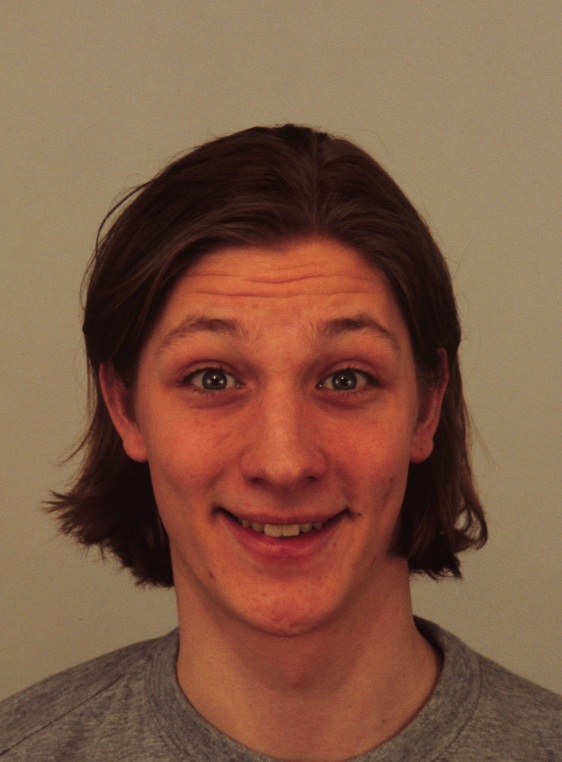
\includegraphics[scale=0.2]{exercise_3/paper/images/AM18HAS.JPG}
                    \caption{Face classified as happy by the Azure Emotion API}
                    \label{fig:happy_face}
            \end{figure}
        
        In the Microsoft Azure Emotion API there is a free pricing option which allows us to submit up to 20 images per minute as well as a premium plan with up to 10 calls per second. As Microsoft has a promotion for students, which gives 100€ free credit, we chose the premium plan. %which allows us to submit up to 10 images per second.
        
        We decided to steal the model behind this API because this is also considered in the paper by Correia-Silva et al.~\cite{copycat}. Hence, we are able to assess whether the performance of our extracted classifier is similar to the performance of the extracted classifier in the paper.
        
       As mentioned in the beginning of Section~\ref{sec:copycat} Azure could not recognise all of the faces in our data set and hence could not classify for each face an emotion. Therefore, we added to the 8 emotions a further class called 'no\textunderscore face'.
        
        %Originally, we wanted to add instances, which are not part of the problem domain to our fake data set. However, as Azure does not classify images in which it does not detect any face, this was not possible.
        
    \subsection{Evaluation 1}
        Since we had labeled data, we were able to compute the accuracy of the Microsoft Azure Emotion API. On the whole data set we obtained an accuracy of $0.76$.
        
        For testing the efficiency of our extracted model, we initially did a $75\%/25\%$ training/test split on our data set consisting of KDEF, AKDEF and the one from Kaggle. As we had labeled data, we had to delete the labels before querying the Azure API as a black-box. From now on we will refer to the training set as attack set, since this set will be used to attack the target network.
        
        To learn the effect of the number if images in the training set, we used an incremental approach. We trained the model on progressively larger subsets of the training set, which were included in each other. Starting with a random sample $s_0$ of $2\,000$ images, the next training set $s_n$ consisted of $s_{n-1}$ and additional $1\,000$ images.
        
        In order to compare the performance of our extracted models to the target network we considered two measures:
        \begin{itemize}
            \item Accuracy: correctly classified faces with respect to the original labels.
            \item Equality: correctly classified faces with respect to the target network.  
        \end{itemize}
        %The CNN-classifier was trained by a Multi-layer Perceptron. As the copying algorithm used for this classifier was rather basic we mapped the size of the training set to the size of the subset of AKDEF/KDEF used to train our copy-cat.
        
        %In order to compare the performance of our copied classifier to the original we split the data set into a test and training set and looked at the accuracy resp. equality of our copied model, dependant on the size of the set used to train the model. We trained the model on progressively larger subsets of the training set, which were included in each other. 
        
        Figure~\ref{fig:performance-azure} shows the results of our tests. Overall it can be seen that the accuracy as well as the equality improve for larger training sets. The best value for the accuracy in our tests was $0.578$. which seems much better compared to the results from the paper with about $0.35$. We also computed the accuracy of the Azure Emotion API on the test set and obtained an accuracy of $0.764$.
        
        However, the extracted model using the whole training set was was able to coincide on $70\%$ on the test data. 
        
        \begin{figure}[h!]
            \centering
            \begin{subfigure}[c]{0.49\textwidth}
                \centering
                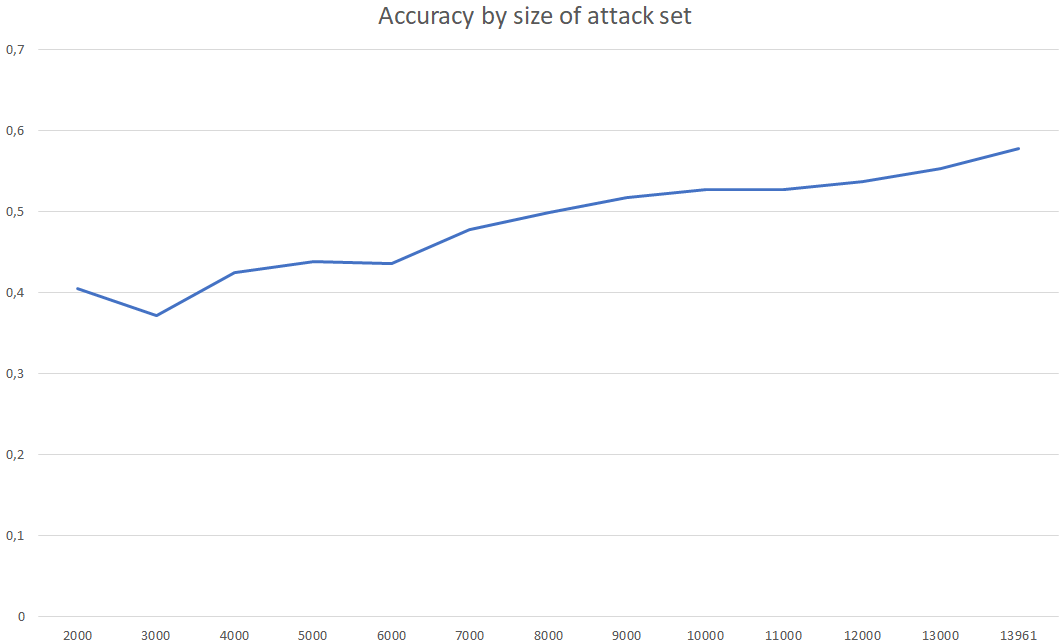
\includegraphics[width=1\textwidth]{exercise_3/paper/images/accuracy_copy_Azure.png}
                \caption{Accuracy of the extracted models}
                \label{fig:Accuracy_Azure}
            \end{subfigure}
            \begin{subfigure}[c]{0.49\textwidth}
                \centering
                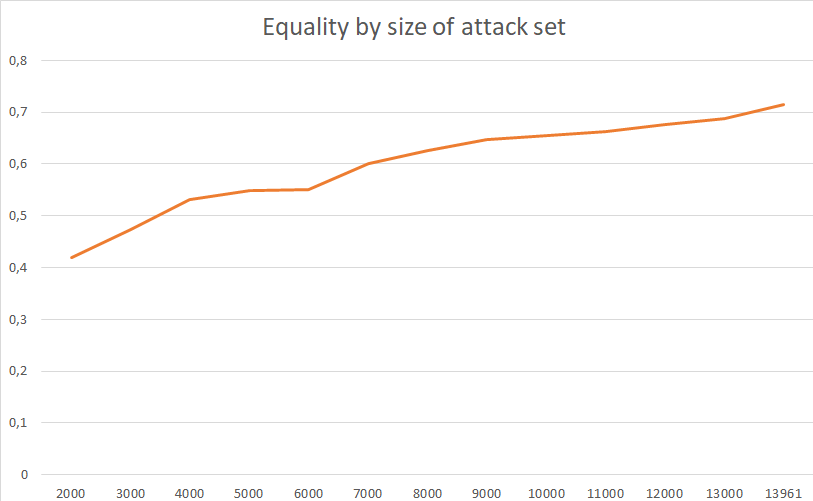
\includegraphics[width=1\textwidth]{exercise_3/paper/images/equality_copy_Azure.png}
                \caption{Equality of the extracted models}
                \label{fig:Equality_Azure}
            \end{subfigure}
            \caption{Performance of Copycat Attack on first data set}
            \label{fig:performance-azure}
        \end{figure}
    The training of the biggest copied model took only roughly one hour, including the time needed to question the Azure API on the labeling of our data set. This was in part to the offer allowing students to get $100$\$ of credit for free and therefore letting us to label $10$ images per second. Had we used the free tier we would have needed roughly $16$ hours of time which is still a reasonable timeframe.
    \subsection{Second Data Set}
        In the following problem, we want to predict if a certain image contains a cat, a dog or none of them. 
        
        For building a model we will again combine several data sets. First of all, we need a training set for training the target network. Additionally, we will need images for the attack resp. test set. 
        
        \subsubsection{Cat data set}
            %https://www.kaggle.com/crawford/cat-dataset 9000 Bilder 
            This data set taken from \hyperlink{https://archive.org/details/CAT_DATASET}{archive.org} contains roughly $10\,000$ images of cats in various positions. Additionally pointers to the eyes, ears and nose of the cats were given, however we did not use them in any capacity. 
            
        \subsubsection{Stanford dogs data set }
            The data set was built using images from ImageNet, by \hyperlink{http://vision.stanford.edu/aditya86/ImageNetDogs/}{Stanford university} , in order to help categorize images. It contains $20\,580$ pictures of dogs. It theoretically contains classifications for different breeds of dogs, but once again we did not use this.
            
        \subsubsection{Common objects in context data set}
            Since our model for this exercise was homemade, we could use copy-cat to it's full power and include non-domain data in our training set for our copy-cat model. For this we chose a dataset from \hyperlink{https://cocodataset.org/\#download}{Common objects in context} containing $118\,000$ images of trains.
            
        
     \subsection{Dogs vs. Cats}
            For the second attempt we chose to train our own CNN to steal to make matters more interesting. We trained our model using the following competition data set from \hyperlink{https://www.kaggle.com/c/dogs-vs-cats/data}{Kaggle}. 
\section{last classifier}



\section{Conclusions}

\bibliographystyle{abbrv}
\bibliography{literature}

\end{document}